% Standalone TikZ figure — compile with: pdflatex pipeline.tex
\documentclass[tikz,border=2pt]{standalone}
\usepackage{tikz}
\usetikzlibrary{arrows.meta, positioning, shapes.geometric}

\begin{document}
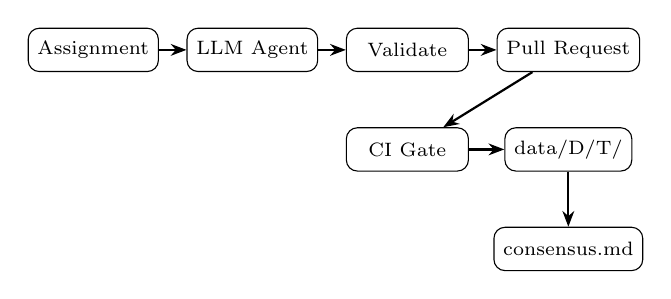
\begin{tikzpicture}[
  node distance=0.55cm and 0.35cm,
  box/.style={draw, rounded corners, align=center, font=\scriptsize,
              minimum width=1.55cm, minimum height=0.55cm},
  arr/.style={-{Stealth[length=2mm]}, thick}
]
  \node[box] (assign) {Assignment};
  \node[box, right=of assign] (agent) {LLM Agent};
  \node[box, right=of agent] (valid) {Validate};
  \node[box, right=of valid] (pr) {Pull Request};
  \node[box, below=0.7cm of valid] (ci) {CI Gate};
  \node[box, below=0.7cm of pr] (ledger) {data/D/T/};
  \node[box, below=0.7cm of ledger] (cons) {consensus.md};

  \draw[arr] (assign) -- (agent);
  \draw[arr] (agent) -- (valid);
  \draw[arr] (valid) -- (pr);
  \draw[arr] (pr) -- (ci);
  \draw[arr] (ci) -- (ledger);
  \draw[arr] (ledger) -- (cons);
\end{tikzpicture}
\end{document}
